\documentclass[a4paper]{article}
\usepackage{student}

% PREENCHA ESSA PARTE COM SEUS DADOS

\setuniversity{UNIVERSIDADE DO ESTADO DE SANTA CATARINA}
\setdepartment{CENTRO DE EDUCAÇÃO DO PLANALTO NORTE/DEPARTAMENTO DE SISTEMAS DE INFORMAÇÃO}
\setmodule{ROTEIRO DE ATIVIDADES ESP-32 e IoT}
\setterm{2025/5° FASE}

\title{AUTOMAÇÃO DE SISTEMAS}
\setmembername{ACELINO MARGOTTI, LUIS FERNANDO MUNHOZ, TIAGO MEIRIB, VITOR KNOP.}
\setmemberuid{2070312308, 2070312320, 2070312209, 2070312231.}

\usepackage{amsmath,amssymb,bm}
\usepackage{hyperref}
\usepackage[T1]{fontenc}


\begin{document}

    \header{}
    % UTILIZAR O AMBIENTE "answer" para criar uma nova caixa de resposta
    % O texto entre chaves [] será utilizado como título antes da caixa
    % Exemplo abaixo:
    
    \begin{answer}[1. Introdução ao ESP32 e Conceitos de IoT]
    \begin{enumerate}
        \item O que é o microcontrolador?
         
            Um microcontrolador é um circuito integrado que contém um processador, 
            memória e periféricos de entrada/saída em um único chip, sendo utilizado
            para controlar dispositivos eletrônicos de forma autônoma.

        \item Diferença entre ESP8266, ESP32 e Arduino Uno.
        
            O ESP8266 é um microcontrolador com conectividade Wi-Fi, enquanto o ESP32
            é uma versão mais avançada com Wi-Fi e Bluetooth integrados, oferecendo
            mais recursos e potência de processamento. O Arduino Uno é uma placa
            de prototipagem baseada no microcontrolador ATmega328, que não possui
            conectividade Wi-Fi ou Bluetooth nativa, mas é amplamente utilizado
            para projetos de eletrônica e programação básica.

        \item Conceitos básicos de Internet das Coisas (IoT).
        
            Internet das Coisas (IoT) refere-se à interconexão de dispositivos físicos
            à internet, permitindo que eles coletem e compartilhem dados, além de
            serem controlados remotamente. Isso possibilita a automação, monitoramento
            e otimização de processos em diversas áreas, como residências, indústrias
            e cidades inteligentes.
        
        \item Exemplos de aplicações com ESP32 e IoT.
            O ESP32 pode ser utilizado em diversas aplicações de IoT, como:

            \begin{itemize}
                \item Monitoramento ambiental (temperatura, umidade, qualidade do ar);
                \item Automação residencial (controle de luzes, eletrodomésticos, sistemas de segurança);
                \item Sistemas de irrigação inteligente;
                \item Dispositivos vestíveis (wearables) para monitoramento de saúde;
                \item Controle remoto de robôs e drones.
            \end{itemize}
    \end{enumerate}
    \end{answer}
    
    \begin{answer}[2. Instalação da IDE Arduino e Configuração do ESP32.]
        \begin{enumerate}
            \item  Instalação da IDE Arduino:

                A IDE Arduino é uma plataforma de desenvolvimento integrada que permite
                programar microcontroladores, incluindo o ESP32. Para instalar a IDE,
                basta baixar o instalador do site oficial do Arduino e seguir as instruções
                de instalação.

                \begin{itemize}
                    \item  Acesse o site oficial do Arduino: \url{https://www.arduino.cc/en/software}.
                    \item  Baixe a versão adequada para o seu sistema operacional (Windows, macOS, Linux).
                    \item  Execute o instalador e siga as instruções na tela.
                    \item  Após a instalação, abra a IDE Arduino.
                \end{itemize}
            \item Configuração do ESP32 na IDE Arduino:
            
                Para programar o ESP32 na IDE Arduino, é necessário instalar o suporte
                ao ESP32. Siga os passos abaixo:

                \begin{itemize}
                    \item  Abra a IDE Arduino.
                    \item  Vá para "File" $>$ "Preferences".
                    \item  Na seção "Additional Boards Manager URLs", adicione a seguinte  URL:
                        \url{https://raw.githubusercontent.com/espressif/arduino-esp32/gh-pages/package_esp32_index.json}.
                    \item  Para facilitar, veja a imagem abaixo mostrando onde adicionar a URL:

                        \begin{center}
                            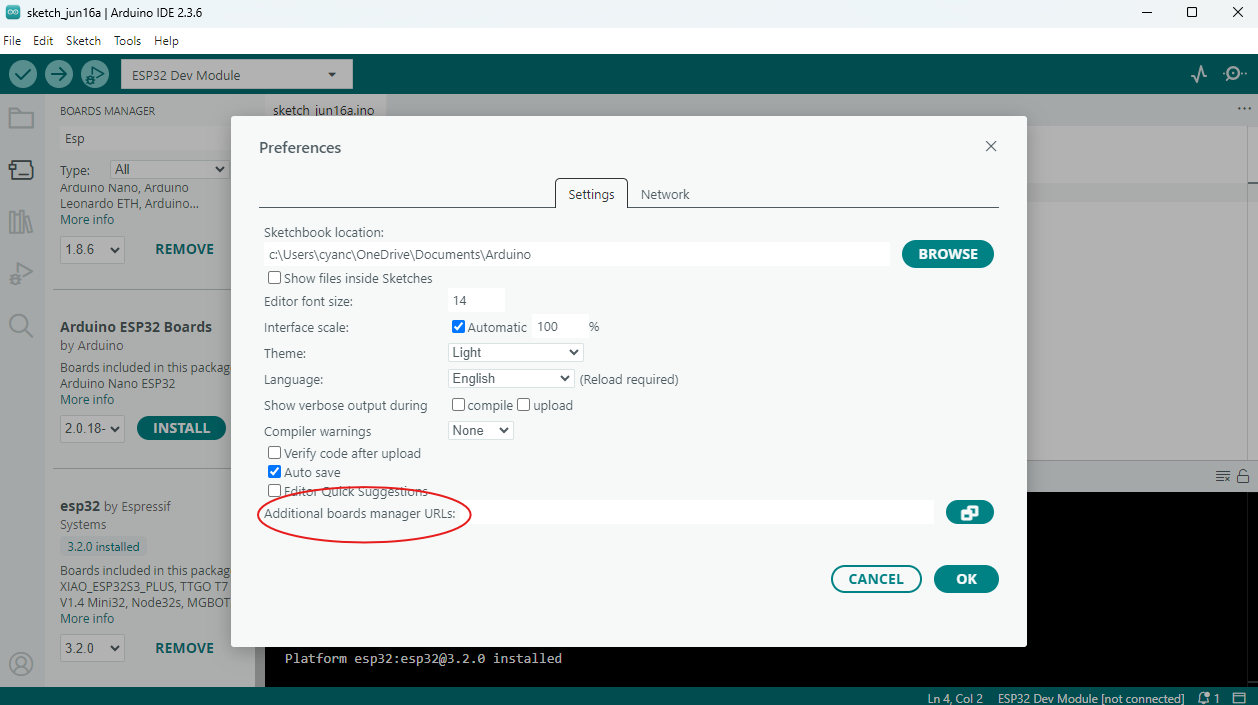
\includegraphics[width=0.7\textwidth]{images/addURL}
                        \end{center}
                    \item  Clique em "OK" para salvar as preferências.
                    \item  Vá para "Tools" $>$ "Board" $>$ "Boards Manager".
                    \item  Pesquise por "ESP32" e instale o pacote "esp32 by Espressif".
                    \item  Veja a imagem abaixo mostrando a seleção da placa:

                        \begin{center}
                            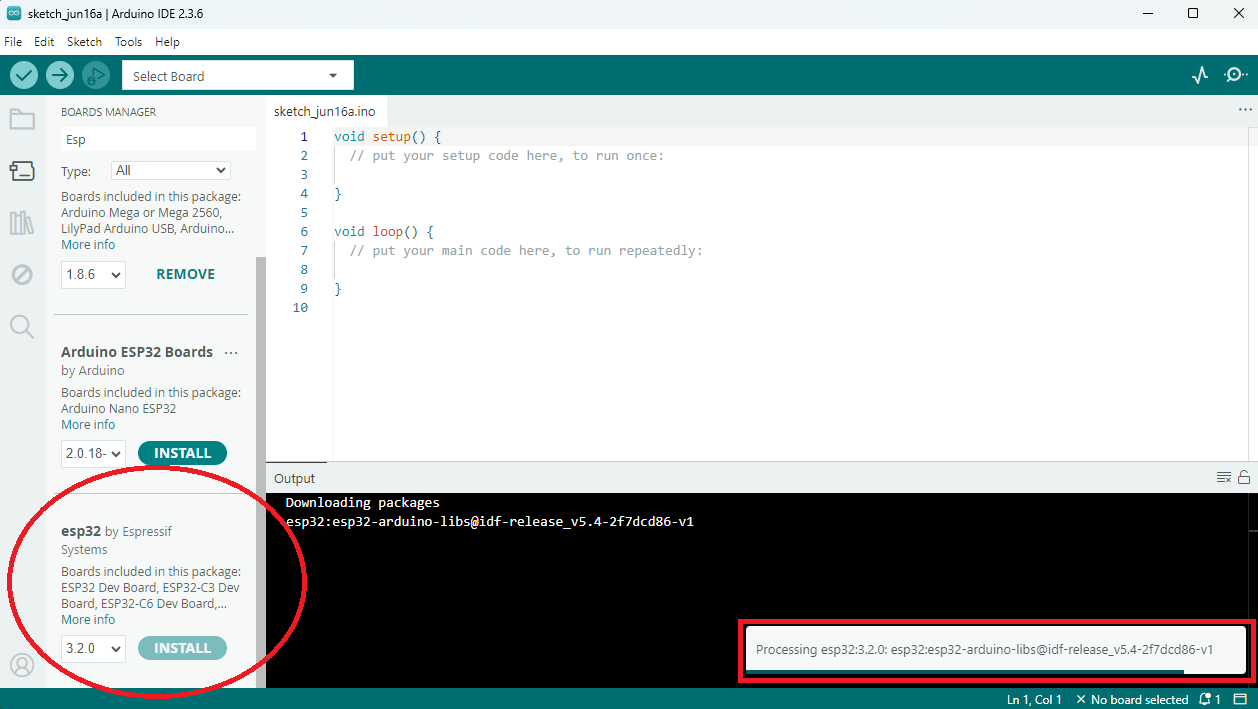
\includegraphics[width=0.7\textwidth]{images/Esp-32-board-install.png}
                        \end{center}
                    \item  Após a instalação, selecione a sua placa ESP32 em "Tools" $>$ "Board".
                    \item  Após instalar o pacote e selecionr a placa, conecte sua placa ESP32 ao computador.
                    \item  Selecione a porta correta em "Tools" $>$ "Port".
                    
                \end{itemize}
            \item  Teste de conexão com código "Blink":

                Para verificar se a configuração está correta, você pode carregar o
                exemplo "Blink" na IDE Arduino. Siga os passos abaixo:

                \begin{itemize}
                    \item  Vá para "File" $>$ "Examples" $>$ "01.Basics" $>$ "Blink".
                    \item  O código do exemplo deve ser semelhante ao seguinte:

                    \begin{verbatim}
                    void setup() {
                        pinMode(LED_BUILTIN, OUTPUT);
                    }

                    void loop() {
                        digitalWrite(LED_BUILTIN, HIGH); // Liga LED
                        delay(1000); // Espera por 1 segundo
                        digitalWrite(LED_BUILTIN, LOW); // Desliga LED
                        delay(1000); // Espera por 1 segundo
                    }
                    \end{verbatim}

                    \item  Carregue o código na placa ESP32 clicando no botão de upload (seta para a direita).
                    \begin{center}
                        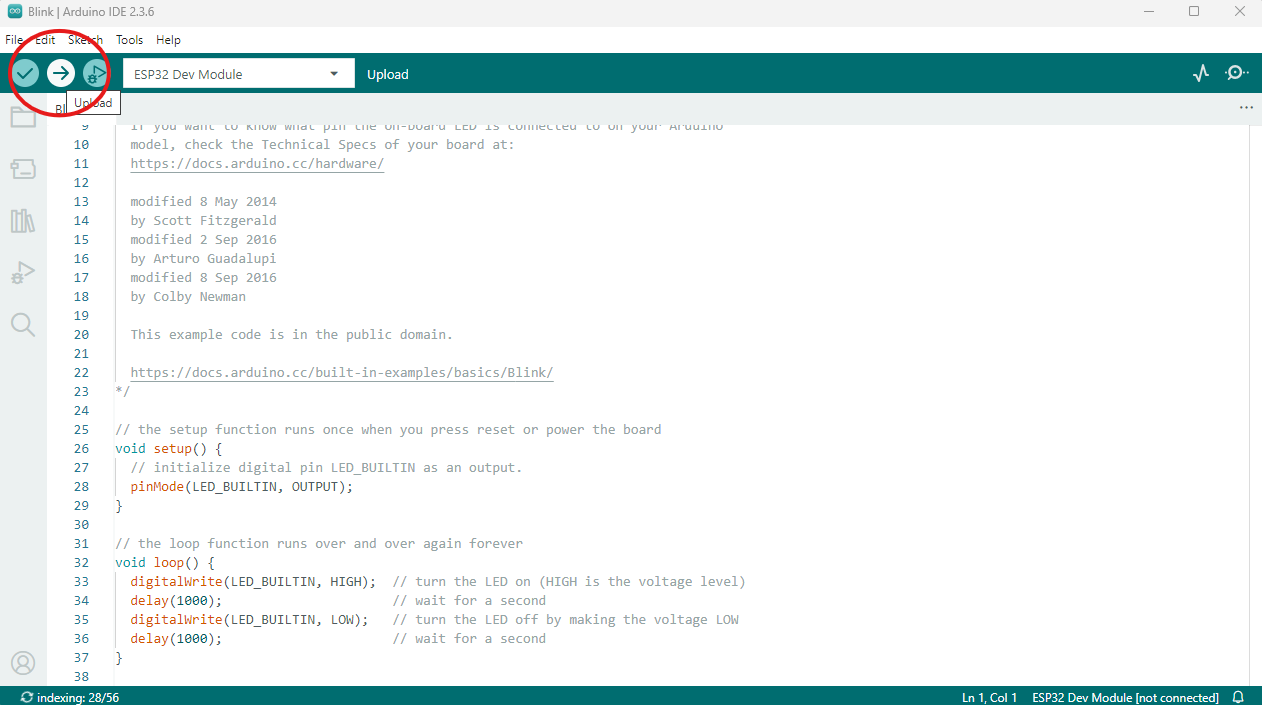
\includegraphics[width=0.7\textwidth]{images/upload.png}
                    \end{center}
                    \item  Após o upload, o LED integrado da placa deve piscar a cada segundo.
                \end{itemize}
        \end{enumerate}
    \end{answer}

    \begin{answer}[3. Comparação com ESP8266 e Arduino Uno.]
        \begin{itemize}
            \item \textbf{ESP32:} Microcontrolador avançado da Espressif, possui processador dual-core, conectividade Wi-Fi e Bluetooth integrados, maior quantidade de pinos de entrada/saída, suporte a múltiplos periféricos, ADCs de maior resolução e maior capacidade de processamento e memória. Ideal para aplicações IoT mais complexas e que exigem conectividade sem fio diversificada.
                \begin{center}
                    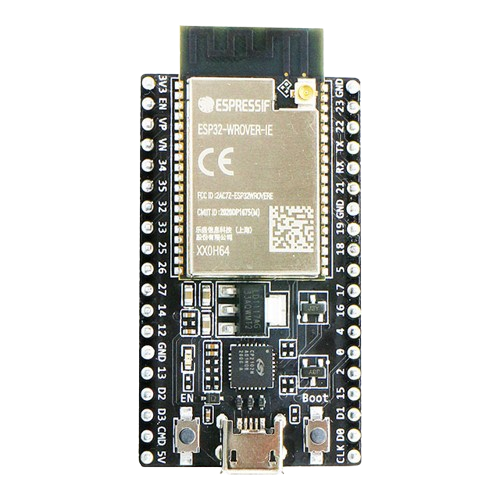
\includegraphics[width=0.5\textwidth]{images/esp32.png}
                \end{center}
            \item \textbf{ESP8266:} Também da Espressif, é mais simples que o ESP32, com processador single-core, conectividade Wi-Fi integrada, menos pinos e recursos. É indicado para projetos IoT básicos que demandam apenas Wi-Fi e menor consumo de recursos.
                \begin{center}
                    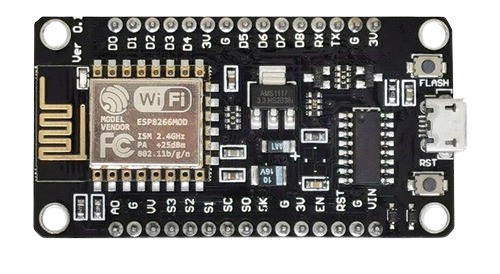
\includegraphics[width=0.5\textwidth]{images/esp8266.png}
                \end{center}
            \item \textbf{Arduino Uno:} Baseado no microcontrolador ATmega328P, não possui conectividade Wi-Fi ou Bluetooth nativa, mas é muito utilizado em projetos de eletrônica básica, prototipagem e ensino. Possui menos memória e processamento em relação aos ESPs, mas conta com vasta documentação e comunidade.
                \begin{center}
                    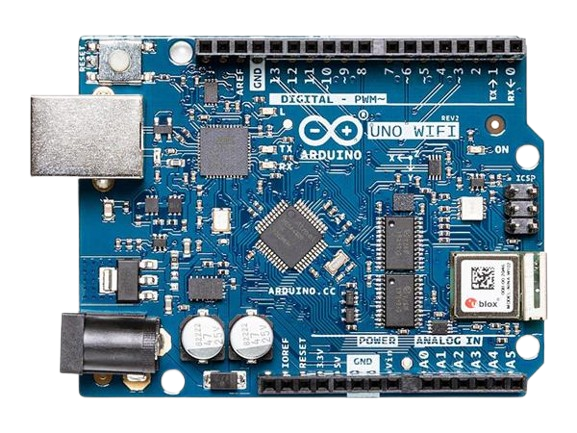
\includegraphics[width=0.5\textwidth]{images/arduino_uno.png}
                \end{center}
        \end{itemize}

        \textbf{Resumo:} O ESP32 é o mais completo em termos de recursos e conectividade, seguido pelo ESP8266 (mais simples e barato), enquanto o Arduino Uno é ideal para projetos básicos sem necessidade de conexão sem fio.
    \end{answer}

    \begin{answer}[4. Leitura de sensores analógicos e digitais]

        Obetivo: Aprender a ler dados de sensores analógicos e digitais utilizando o ESP32.
        \begin{enumerate}
            \item Leitura de sensores analógicos:

                Para ler dados de sensores analógicos, como um potenciômetro ou sensor de temperatura, você pode usar a função `analogRead()`. O ESP32 possui vários pinos ADC (Conversores Analógico-Digital) que podem ser utilizados para essa finalidade.

                Exemplo de código para ler um sensor analógico:

            \begin{verbatim}
            int sensorPin = 34; // Pino ADC
            int sensorValue = 0;

            void setup() {
                Serial.begin(115200);
            }

            void loop() {
                sensorValue = analogRead(sensorPin); // Lê o valor do sensor
                Serial.println(sensorValue); // Imprime o valor no monitor serial
                delay(1000); // Espera 1 segundo
            }
            \end{verbatim}

            \item Leitura de sensores digitais:

                Para ler dados de sensores digitais, como um botão ou sensor de movimento, você pode usar a função `digitalRead()`. O ESP32 possui vários pinos digitais que podem ser utilizados para essa finalidade.

                Exemplo de código para ler um sensor digital:

            \begin{verbatim}
            int buttonPin = 2; // Pino digital
            int buttonState = 0;

            void setup() {
                pinMode(buttonPin, INPUT); // Configura o pino como entrada
                Serial.begin(115200);
            }

            void loop() {
                buttonState = digitalRead(buttonPin); // Lê o estado do botão
                Serial.println(buttonState); // Imprime o estado no monitor serial
                delay(1000); // Espera 1 segundo
            }
            \end{verbatim}
        \end{enumerate}
    \end{answer}

    \begin{answer}[5. Controle de atuadores (EX: LED e buzzer).]
        \begin{enumerate}
            \item Controle de LED:

                Para controlar um LED, você pode usar a função `digitalWrite()`. O ESP32 possui vários pinos digitais que podem ser utilizados para essa finalidade.

                Exemplo de código para controlar um LED:

            \begin{verbatim}
            int ledPin = 2; // Pino do LED

            void setup() {
                pinMode(ledPin, OUTPUT); // Configura o pino como saída
            }

            void loop() {
                digitalWrite(ledPin, HIGH); // Liga o LED
                delay(1000); // Espera 1 segundo
                digitalWrite(ledPin, LOW); // Desliga o LED
                delay(1000); // Espera 1 segundo
            }
            \end{verbatim}
            O resultado será um LED piscando a cada segundo (Conforme a imagem abaixo).
            \begin{center}
                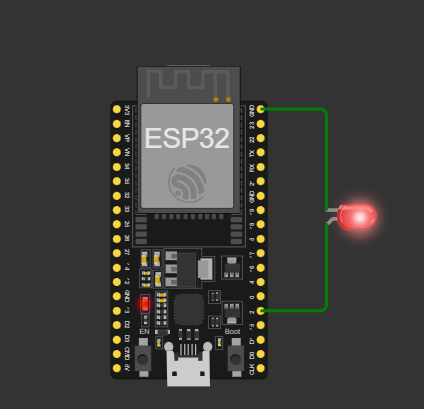
\includegraphics[width=0.5\textwidth]{images/led.png}
            \end{center}
            \begin{center}
                \small
                \textbf{Figura:} Imagem retirada do simulador ESP32 \href{https://wokwi.com}{wokwi.com}.
            \end{center}

            \item Controle de buzzer:

                Para controlar um buzzer, você também pode usar a função `digitalWrite()`.

                Exemplo de código para controlar um buzzer:

            \begin{verbatim}
            int buzzerPin = 2; // Pino do buzzer

            void setup() {
                pinMode(buzzerPin, OUTPUT); // Configura o pino como saída
            }

            void loop() {
                // Aumenta a frequência gradualmente (efeito de sirene)
                for (int freq = 800; freq <= 2000; freq += 10) {
                    tone(buzzerPin, freq); // Gera tom com a frequência atual
                    delay(10); // Pequeno atraso para suavizar a transição
                }
                
                // Diminui a frequência gradualmente
                for (int freq = 2000; freq >= 800; freq -= 10) {
                    tone(buzzerPin, freq); // Gera tom com a frequência atual
                    delay(10); // Pequeno atraso para suavizar a transição
                }
                
                noTone(buzzerPin); // Para o som
                delay(200); // Pausa breve antes de reiniciar
                }
            \end{verbatim}
            O resultado será um buzzer emitindo um som de sirene (visualmente conforme a imagem abaixo).
            \begin{center}
                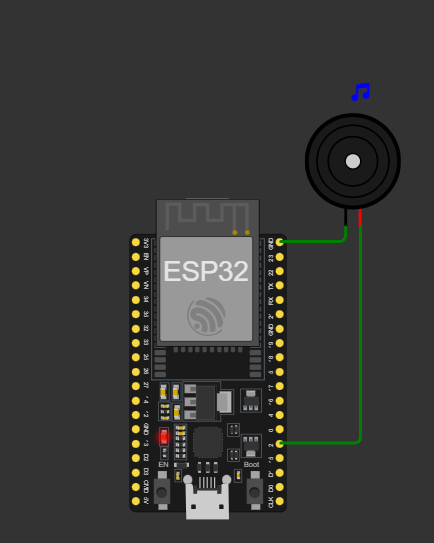
\includegraphics[width=0.5\textwidth]{images/buzzer.png}
            \end{center}
            \begin{center}
                \small
                \textbf{Figura:} Imagem retirada do simulador ESP32 \href{https://wokwi.com}{wokwi.com}.
            \end{center}
        \end{enumerate}
    \end{answer}

    \begin{answer}[6. Conectando o ESP32 a uma rede Wi-Fi.]
        \begin{enumerate}
            \item Biblioteca WiFi\.h:
            
            Para conectar o ESP32 a uma rede Wi-Fi, utilizamos a biblioteca WiFi.h, que já vem incluída no pacote ESP32 da IDE Arduino. Esta biblioteca fornece todas as funções necessárias para gerenciar conexões Wi-Fi..

            \begin{verbatim}
            #include <WiFi.h>
            \end{verbatim}

            \item Configuração básica de conexão Wi-Fi:

                Exemplo básico de como conectar o ESP32 a uma rede Wi-Fi fornecendo o SSID e senha:

            \begin{verbatim}
            #include <WiFi.h>

            const char* ssid = "NOME_DA_SUA_REDE";
            const char* password = "SENHA_DA_SUA_REDE";

            void setup() {
                Serial.begin(115200);

                WiFi.begin(ssid, password);
                Serial.print("Conectando à rede Wi-Fi");

                while (WiFi.status() != WL_CONNECTED) {
                    delay(1000);
                    Serial.print(".");
                }

                Serial.println();
                Serial.println("Conectado com sucesso!");
                Serial.print("Endereço IP: ");
                Serial.println(WiFi.localIP());
            }

            void loop() {
            // Código principal aqui
            }

            \end{verbatim}
        
            \item Verificação do status da conexão:

                Código para verificar o status da conexão e exibir informações sobre a rede Wi-Fi:
            \begin{verbatim}
                #include <WiFi.h>

                const char* ssid = "NOME_DA_SUA_REDE";
                const char* password = "SENHA_DA_SUA_REDE";

                void setup() {
                Serial.begin(115200);

                WiFi.begin(ssid, password);
                Serial.print("Conectando à rede Wi-Fi");

                int tentativas = 0;
                while (WiFi.status() != WL_CONNECTED && tentativas < 20) {
                    delay(1000);
                    Serial.print(".");
                    tentativas++;
                }

                if (WiFi.status() == WL_CONNECTED) {
                    Serial.println();
                    Serial.println("Conectado com sucesso!");
                    Serial.print("SSID: ");
                    Serial.println(WiFi.SSID());
                    Serial.print("Endereço IP: ");
                    Serial.println(WiFi.localIP());
                    Serial.print("Intensidade do sinal (RSSI): ");
                    Serial.println(WiFi.RSSI());
                } else {
                    Serial.println();
                    Serial.println("Falha na conexão Wi-Fi!");
                    Serial.println("Verifique as credenciais da rede.");
                }
                }

                void loop() {
                if (WiFi.status() == WL_CONNECTED) {
                    Serial.println("Wi-Fi conectado");
                } else {
                    Serial.println("Wi-Fi desconectado - tentando reconectar...");
                    WiFi.begin(ssid, password);
                }

                delay(10000);
                }
            \end{verbatim}
        
            \item Códigos de status Wi-Fi:

                Principais códigos de status retornados por WiFi.status():
                    \begin{itemize}
                        \item \texttt{WL\_CONNECTED} (3): Conectado com sucesso.
                        \item \texttt{WL\_NO\_SSID\_AVAIL} (1): SSID não encontrado.
                        \item \texttt{WL\_CONNECT\_FAILED}: (4) Falha na conexão por senha incorreta.   
                        \item \texttt{WL\_CONNECTION\_LOST}: A conexão com a rede Wi-Fi foi perdida.
                        \item \texttt{WL\_DISCONNECTED}: O ESP32 está desconectado da rede Wi-Fi.
                    \end{itemize}
            
            \item Exemplo completo com reconexão automática:

                Código completo com reconexão automática à rede Wi-Fi:
            \begin{verbatim}
                #include <WiFi.h>

                const char* ssid = "NOME_DA_SUA_REDE";
                const char* password = "SENHA_DA_SUA_REDE";

                void conectarWiFi() {
                WiFi.begin(ssid, password);

                Serial.print("Conectando à rede Wi-Fi");

                int tentativas = 0;
                while (WiFi.status() != WL_CONNECTED && tentativas < 20) {
                    delay(1000);
                    Serial.print(".");
                    tentativas++;
                }

                if (WiFi.status() == WL_CONNECTED) {
                    Serial.println();
                    Serial.println("OK Conectado com sucesso!");
                    exibirInformacoesRede();
                } else {
                    Serial.println();
                    Serial.println("X Falha na conexão Wi-Fi!");
                }
                }

                void exibirInformacoesRede() {
                    Serial.println("=== Informações da Rede ===");
                    Serial.print("SSID: ");
                    Serial.println(WiFi.SSID());
                    Serial.print("Endereço IP: ");
                    Serial.println(WiFi.localIP());
                    Serial.print("Gateway: ");
                    Serial.println(WiFi.gatewayIP());
                    Serial.print("Máscara de sub-rede: ");
                    Serial.println(WiFi.subnetMask());
                    Serial.print("DNS: ");
                    Serial.println(WiFi.dnsIP());
                    Serial.print("Intensidade do sinal (RSSI): ");
                    Serial.print(WiFi.RSSI());
                    Serial.println(" dBm");
                    Serial.println("===========================");
                }

                void setup() {
                    Serial.begin(115200);
                    WiFi.mode(WIFI_STA);
                    conectarWiFi();
                }

                void loop() {
                if (WiFi.status() != WL_CONNECTED) {
                    Serial.println("Conexão Wi-Fi perdida. Tentando reconectar...");
                    conectarWiFi();
                } else {
                    Serial.println("Wi-Fi conectado - Sistema funcionando normalmente");
                }

                delay(30000);
                }
            \end{verbatim}
        
            \item Explicação do código:

                Dicas importantes:
                \begin{itemize}
                        \item \texttt Substitua as credenciais da rede pelos seus dados reais.
                        \item \texttt RSSI próximo de 0 indica sinal forte. Mais negativo = mais fraco.
                        \item \texttt{WiFi.mode(WIFI\_STA)} configura o ESP32 como cliente Wi-Fi.
                        \item Outros modos: \texttt{WIFI\_AP} (Access Point), \texttt{WIFI\_AP\_STA} (modo misto).
                        \item \texttt Definir limite de tentativas evita travamento se a rede estiver indisponível.
                    \end{itemize}

            \item Testando a conexão:
            
                \begin{itemize}
                    \item \texttt Após carregar o código, abra o Monitor Serial (Ctrl+Shift+M).
                    \item \texttt Configure para 115200 baud.
                    \item \texttt Veja as mensagens de conexão e o IP atribuído ao ESP32.
                \end{itemize}

            Com o ESP32 conectado, é possível comunicar com outros dispositivos e com a Internet usando protocolos como MQTT.
        \end{enumerate}
    \end{answer}

    \begin{answer}[7. Introdução ao protocolo MQTT.]
        O protocolo MQTT é o protocolo padrão pra comunicação entre dispositivos IoT. Ele é
        planejado pra ser extremamente leve, com o padrão de publicador / assinante que é ideal pra
        conectar dispositivos com o mínimo de recursos possível. Ele é usado em diversas indústrias,
        como automotiva, manufatura, telecomunicação, entre outras.

        \begin{enumerate}
            \item O padrão da indústria:
            
                Ele é o protocolo mais usado na indústria, porque é o que melhor funciona em dispositivos com
                recursos limitados, com baixa largura de banda e conectividade limitada. Ele usa por baixo dos
                panos o TCP/IP, com um formato de mensagem binária, em contraste com outros protocolos
                que usam um formato de mensagens de texto, como o HTTP, saindo na frente no transporte de
                dados.
            
            \item Modelo Publicador / Assinante:
            \begin{itemize}
                    \item \texttt Publicadores (publishers) enviam mensagens em tópicos.
                    \item \texttt Assinantes (subscribers) recebem mensagens do tópico que assinaram.
                    \item \texttt Um broker (servidor intermediário) gerencia o envio das mensagens aos clientes.
                \end{itemize}
            
            É assim que funciona a comunicação entre os dispositivos com o protocolo MQTT. Ele também
            tem outras funcionalidades interessantes, como a de sessões persistentes: se a sessão entre
            um publicador / assinante for desconectada, a sessão vai continuar ativa mesmo assim. Uma
            vez que a internet for conectada novamente, eles vão se conectar de novo automaticamente e
            continuar a sessão.

            Também existem outras opções que o MQTT oferece:

            \begin{itemize}
                    \item \texttt {Retenção de mensagens:}  É possível configurar mensagens como "retidas", assim quando novos assinantes assinam um tópico, eles recebem imediatamente a última mensagem publicada.
                    \item \texttt {Qualidade de serviço (QoS):}Oferece três níveis de entrega de mensagens:
                        \begin{itemize}
                            \item QoS 0: Entrega no mínimo uma vez (sem garantia de entrega).
                            \item QoS 1: Entrega pelo menos uma vez (pode haver duplicação).
                            \item QoS 2: Entrega exatamente uma vez (garantia de entrega sem duplicação).
                        \end{itemize}
                    \item \texttt {Mensagens com última vontade (Last will and testament):} Permite que o cliente defina uma mensagem que será enviada se ele se desconectar de forma inesperada. É útil pra detectar falhas em dispositivos.
                \end{itemize}

        \end{enumerate}

    \end{answer}

    \begin{answer}[8. Publicando dados do sensor em um broker MQTT.]
        Como Publicar Dados de um Sensor em um Broker MQTT Usando um ESP32:

        O protocolo MQTT (Message Queuing Telemetry Transport) é ideal para aplicações de IoT devido à sua leveza e eficiência. Com um ESP32, é possível coletar dados de um sensor e publicá-los em um broker MQTT de forma simples. Abaixo estão os passos para configurar e implementar essa tarefa.

        \begin{enumerate}
            \item Escolha e Configure o Broker MQTT:
            
            O broker MQTT é o servidor que gerencia as mensagens entre dispositivos. Você pode usar:
                \begin{itemize}
                    \item \textbf{Broker local:} Instale o Mosquitto em um computador ou servidor:
                    \begin{verbatim}
                    sudo apt-get install mosquitto mosquitto-clients
                    \end{verbatim}
                    \item \textbf{Broker na nuvem:} Serviços como HiveMQ Cloud ou Adafruit IO são boas opções. Crie uma conta para obter o endereço do broker, porta (geralmente 1883 para conexões não seguras ou 8883 para TLS), usuário e senha (se necessário).
                    \item Certifique-se de que o broker está acessível e as portas estão abertas.
                \end{itemize}
            
            \item Conecte o Sensor ao ESP32:
            Conecte o sensor ao ESP32. Neste exemplo, usaremos um sensor de temperatura e umidade DHT11:
            \begin{itemize}
                \item \textbf{Pino de dados do DHT11:} Conecte a um pino GPIO, como o GPIO 4.
                \item \textbf{Alimentação:} Conecte VCC ao 3,3V e GND ao GND do ESP32.
                \item Adicione um resistor pull-up de $4.7\,\mathrm{k}\Omega$ a $10\,\mathrm{k}\Omega$ entre o pino de dados e o VCC, se necessário.
                \item Instale a biblioteca DHT sensor library no Arduino IDE para facilitar a leitura do sensor.
            \end{itemize}

            \item Configure o Ambiente de Programação:
            
            \begin{itemize}
                \item \textbf{Arduino IDE:} Instale o suporte ao ESP32 no Arduino IDE (em "Placas" > "Gerenciador de Placas", procure por "ESP32").
                \item \textbf{Bibliotecas:} Instale as bibliotecas PubSubClient (para MQTT) e WiFi (já inclusa no suporte ao ESP32).
                \item Configure o Wi-Fi do ESP32 com o SSID e a senha da sua rede.
            \end{itemize}

            \item Escreva o Código para o ESP32:
            
            O código abaixo lê a temperatura do sensor DHT11 e a publica em um tópico MQTT. Substitua as variáveis com suas configurações específicas:
            \begin{verbatim}
            #include <WiFi.h>
            #include <PubSubClient.h>
            #include <DHT.h>

            // Configurações de Wi-Fi
            const char* ssid = "SUA_REDE_WIFI";
            const char* password = "SUA_SENHA_WIFI";

            // Configurações do broker MQTT
            const char* mqtt_server = "SEU_BROKER_MQTT"; // ex: broker.hivemq.com
            const int mqtt_port = 1883;
            const char* mqtt_user = "SEU_USUARIO"; // Opcional
            const char* mqtt_password = "SUA_SENHA"; // Opcional
            const char* mqtt_topic = "esp32/temperatura";

            // Configurações do sensor DHT
            #define DHTPIN 4 // Pino GPIO conectado ao DHT11
            #define DHTTYPE DHT11
            DHT dht(DHTPIN, DHTTYPE);

            WiFiClient espClient;
            PubSubClient client(espClient);

            void setup() {
                Serial.begin(115200);
                dht.begin();

                // Conectar ao Wi-Fi
                WiFi.begin(ssid, password);
                while (WiFi.status() != WL_CONNECTED) {
                    delay(1000);
                    Serial.println("Conectando ao WiFi...");
                }
                Serial.println("Conectado ao WiFi");

                // Configurar o broker MQTT
                client.setServer(mqtt_server, mqtt_port);
                }

            void reconnect() {
                while (!client.connected()) {
                    Serial.println("Conectando ao broker MQTT...");
                    String clientId = "ESP32Client-" + String(random(0xffff), HEX);
                    if (client.connect(clientId.c_str(), mqtt_user, mqtt_password)) {
                        Serial.println("Conectado ao broker MQTT");
                    } else {
                        Serial.print("Falha na conexão, rc=");
                        Serial.print(client.state());
                        delay(5000);
                    }
                }
            }

            void loop() {
                if (!client.connected()) {
                    reconnect();
                }
                client.loop();

                // Ler dados do sensor
                float temperatura = dht.readTemperature();
                if (isnan(temperatura)) {
                    Serial.println("Erro ao ler o sensor DHT11!");
                    delay(2000);
                    return;
                }

                // Publicar dados no tópico
                String payload = String(temperatura);
                client.publish(mqtt_topic, payload.c_str());
                Serial.println("Temperatura publicada: " + payload + " °C");

                delay(5000); // Publica a cada 5 segundos
            }
            \end{verbatim}

            \item Escolha do Tópico:
            
            Escolha um tópico descritivo, como esp32/temperatura. Tópicos são organizados hierarquicamente (ex.: dispositivo/local/variável) para facilitar o gerenciamento.

            \item Teste a Publicação:
            \begin{itemize}
                \item \textbf{Carregue o código:} Use o Arduino IDE para compilar e carregar o código no ESP32.
                \item \textbf{Monitore via Serial:} Abra o Monitor Serial (115200 baud) para verificar a conexão Wi-Fi, a conexão com o broker e os dados do sensor.
                \item \textbf{Verifique os dados no broker:} Use um cliente MQTT (como MQTT Explorer ou o comando \texttt{mosquitto\_sub}) para assinar o tópico e confirmar a recepção dos dados:
                \begin{verbatim}
                mosquitto_sub -h SEU_BROKER -t esp32/temperatura
                \end{verbatim}
            \end{itemize}

            \item Segurança (Opcional):
            
            Para Maior segurança:
            \begin{itemize}
                \item Use MQTT com TLS/SSL (porta 8883) e configure certificados no ESP32.
                \item Adicione autenticação com usuário e senha no broker.
                \item Considere criptografar os dados do sensor, se necessário.
            \end{itemize}

            \item Dicas Adicionais:
            \begin{itemize}
                \item \textbf{Qualidade de Serviço (QoS):} No método client.publish, você pode especificar o nível de QoS (0, 1 ou 2) como um parâmetro adicional, dependendo da confiabilidade desejada.
                \item \textbf{Reconexão automática:} O código inclui uma função reconnect() para lidar com desconexões.
                \item \textbf{Outros sensores:} Para sensores diferentes (como BMP280 ou DS18B20), ajuste a leitura no código, mantendo a estrutura de publicação MQTT.
            \end{itemize}

            \item Conclusão:
            
            Com um ESP32, é possível publicar dados de um sensor em um broker MQTT de forma eficiente usando a biblioteca PubSubClient. O exemplo acima usa um sensor DHT11, mas pode ser adaptado para outros sensores. Teste a conexão, monitore os dados e, se necessário, implemente segurança para aplicações reais. 
                \end{enumerate}
    \end{answer}

    \begin{answer}[9. Recebendo comandos MQTT para controle de atuadores.]
        Recebendo Comandos MQTT para Controle de Atuadores com ESP32

        O protocolo MQTT, descrito na página 11 do documento, opera no modelo publicador/assinante, permitindo que dispositivos como o ESP32 publiquem dados em tópicos e assinem tópicos para receber mensagens. Para controlar atuadores (como LEDs, relés ou motores), o ESP32 pode assinar um tópico MQTT, receber comandos enviados por outro dispositivo ou aplicação e atuar sobre um pino GPIO com base nesses comandos. Este texto explica como configurar o ESP32 para receber comandos MQTT e controlar um atuador, usando como exemplo um LED conectado a um pino GPIO.

        \begin{enumerate}

            \item {Pré-requisitos}

            Antes de começar, certifique-se de que:
            \begin{itemize}
                \item O ambiente do Arduino IDE está configurado para o ESP32.
                \item O ESP32 está conectado a um sensor e a um atuador (ex.: um LED conectado ao GPIO 5).
                \item Um broker MQTT está configurado (local, como Mosquitto, ou na nuvem, como HiveMQ Cloud), com endereço, porta (1883 ou 8883 para TLS), usuário e senha, se necessário.
                \item As bibliotecas WiFi, PubSubClient e DHT estão instaladas no Arduino IDE.
            \end{itemize}

            \item{Conexão do Atuador ao ESP32}

            Conecte o atuador ao ESP32. Para este exemplo, usaremos um LED:
            \begin{itemize}
                \item \textbf{Pino do LED:} Conecte o ânodo (perna longa) ao GPIO 5 e o cátodo (perna curta) ao GND, com um resistor de 220$\Omega$ a 330$\Omega$ em série para limitar a corrente.
                \item Alternativamente, use um relé ou outro atuador compatível com os níveis de tensão do ESP32 (3,3V para sinais lógicos).
                \item Verifique se o pino escolhido (GPIO 5) suporta saída digital, conforme descrito na página 4 do documento sobre leitura de sensores analógicos e digitais.
            \end{itemize}

            \item{Configuração do Código}

            O código a seguir adapta o exemplo anterior (publicação de dados do sensor DHT11) para incluir a assinatura de um tópico MQTT e o controle de um LED com base em comandos recebidos. O ESP32 assina o tópico \texttt{esp32/comando} para receber mensagens como "ON" ou "OFF" e controla o LED no GPIO 5. A reconexão automática ao Wi-Fi e ao broker MQTT, também é implementada.

            \begin{verbatim}
            #include <WiFi.h>
            #include <PubSubClient.h>
            #include <DHT.h>

            // Configurações de Wi-Fi
            const char* ssid = "NOME_DA_SUA_REDE";
            const char* password = "SENHA_DA_SUA_REDE";

            // Configurações do broker MQTT
            const char* mqtt_server = "SEU_BROKER_MQTT"; // ex.: broker.hivemq.com
            const int mqtt_port = 1883;
            const char* mqtt_user = "SEU_USUARIO"; // Opcional
            const char* mqtt_password = "SUA_SENHA"; // Opcional
            const char* mqtt_topic_sensor = "esp32/temperatura";
            const char* mqtt_topic_comando = "esp32/comando";

            // Configurações do sensor DHT e do atuador
            #define DHTPIN 4 // Pino GPIO conectado ao DHT11
            #define DHTTYPE DHT11
            #define LED_PIN 5 // Pino GPIO conectado ao LED
            DHT dht(DHTPIN, DHTTYPE);

            WiFiClient espClient;
            PubSubClient client(espClient);

            void connectarWiFi() {
            WiFi.begin(ssid, password);
            Serial.print("Conectando à rede Wi-Fi");
            int tentativas = 0;
            while (WiFi.status() != WL_CONNECTED && tentativas < 20) {
                delay(1000);
                Serial.print(".");
                tentativas++;
            }
            if (WiFi.status() == WL_CONNECTED) {
                Serial.println("\nConectado ao Wi-Fi");
            } else {
                Serial.println("\nFalha na conexão Wi-Fi");
            }
            }

            void callback(char* topic, byte* payload, unsigned int length) {
            // Processar mensagem recebida
            String mensagem;
            for (unsigned int i = 0; i < length; i++) {
                mensagem += (char)payload[i];
            }
            Serial.println("Mensagem recebida no tópico [" + String(topic) + "]: " + mensagem);

            // Controlar o LED com base na mensagem
            if (mensagem == "ON") {
                digitalWrite(LED_PIN, HIGH);
                Serial.println("LED ligado");
            } else if (mensagem == "OFF") {
                digitalWrite(LED_PIN, LOW);
                Serial.println("LED desligado");
            }
            }

            void reconnectMQTT() {
            while (!client.connected()) {
                Serial.println("Conectando ao broker MQTT...");
                String clientId = "ESP32Client-" + String(random(0xffff), HEX);
                if (client.connect(clientId.c_str(), mqtt_user, mqtt_password)) {
                Serial.println("Conectado ao broker MQTT");
                // Assinar o tópico de comandos
                client.subscribe(mqtt_topic_comando, 1); // QoS 1
                } else {
                Serial.print("Falha na conexão, rc=");
                Serial.print(client.state());
                delay(5000);
                }
            }
            }

            void setup() {
            Serial.begin(115200);
            dht.begin();
            pinMode(LED_PIN, OUTPUT); // Configurar o pino do LED como saída
            digitalWrite(LED_PIN, LOW); // Iniciar com LED desligado
            connectarWiFi();
            client.setServer(mqtt_server, mqtt_port);
            client.setCallback(callback); // Definir a função de callback para mensagens recebidas
            }

            void loop() {
            if (WiFi.status() != WL_CONNECTED) {
                connectarWiFi();
            }
            if (!client.connected()) {
                reconnectMQTT();
            }
            client.loop();

            // Ler e publicar dados do sensor
            float temperatura = dht.readTemperature();
            if (!isnan(temperatura)) {
                String payload = String(temperatura);
                client.publish(mqtt_topic_sensor, payload.c_str(), true); // QoS 1, mensagem retida
                Serial.println("Temperatura publicada: " + payload + " °C");
            } else {
                Serial.println("Erro ao ler o sensor DHT11!");
            }

            delay(5000); // Publica e verifica mensagens a cada 5 segundos
            }
            \end{verbatim}

            \item{Explicação do Código}

                \begin{itemize}
                    \item \textbf{Configuração inicial:}
                    \begin{itemize}
                        \item O pino do LED (GPIO 5) é configurado como saída com \texttt{pinMode(LED\_PIN, OUTPUT)}.
                        \item A função \texttt{connectarWiFi()} implementa a reconexão automática ao Wi-Fi, com até 20 tentativas.
                    \end{itemize}
                    \item \textbf{Conexão MQTT:}
                    \begin{itemize}
                        \item A função \texttt{reconnectMQTT()} conecta ao broker e assina o tópico \texttt{esp32/comando} com QoS 1.
                        \item A função \texttt{client.setCallback(callback)} define a função que processa mensagens recebidas.
                    \end{itemize}
                    \item \textbf{Leitura do sensor:}
                    \begin{itemize}
                        \item O sensor DHT11 é lido a cada 5 segundos, e a temperatura é publicada no tópico \texttt{esp32/temperatura} com QoS 1 e mensagem retida.
                    \end{itemize}
                    \item \textbf{Processamento de comandos:}
                    \begin{itemize}
                        \item A função \texttt{callback} é chamada quando uma mensagem é recebida no tópico \texttt{esp32/comando}.
                        \item A mensagem é convertida em uma string e comparada com "ON" ou "OFF" para ligar ou desligar o LED usando \texttt{digitalWrite}.
                    \end{itemize}
                    \item \textbf{Tópicos:}
                    \begin{itemize}
                        \item \texttt{esp32/temperatura}: Para publicar dados do sensor.
                        \item \texttt{esp32/comando}: Para receber comandos do atuador.
                    \end{itemize}
                \end{itemize}

            \item{Teste do Controle do Atuador}

                \begin{itemize}
                    \item \textbf{Carregue o código:} Compile e carregue o código no ESP32 usando o Arduino IDE.
                    \item \textbf{Monitore via Serial:} Abra o Monitor Serial (115200 baud) para verificar conexões Wi-Fi e MQTT, leituras do sensor e comandos recebidos.
                    \item \textbf{Envie comandos MQTT:} Use um cliente MQTT (ex.: MQTT Explorer ou \texttt{mosquitto\_pub}) para publicar comandos no tópico \texttt{esp32/comando}:
                    \begin{itemize}
                        \item \texttt{mosquitto\_pub -h SEU\_BROKER -t esp32/comando -m "ON"}
                        \item \texttt{mosquitto\_pub -h SEU\_BROKER -t esp32/comando -m "OFF"}
                    \end{itemize}
                    \item \textbf{Verifique o atuador:} Confirme se o LED liga ou desliga conforme os comandos enviados. No Monitor Serial, você verá mensagens como "LED ligado" ou "LED desligado".
                    \item \textbf{Debug:} Verifique erros no Monitor Serial, como falhas de conexão (\texttt{WL\_NO\_SSID\_AVAIL}, \texttt{WL\_CONNECT\_FAILED}) ou problemas com o broker MQTT (\texttt{client.state()}).
                \end{itemize}

            \item{Protocolo MQTT e Controle de Atuadores}

                O MQTT é ideal para controle de atuadores devido ao seu modelo publicador/assinante:
                \begin{itemize}
                    \item \textbf{Publicadores:} Um dispositivo ou aplicação (ex.: um aplicativo web ou celular) publica comandos como "ON" ou "OFF" no tópico \texttt{esp32/comando}.
                    \item \textbf{Assinantes:} O ESP32 assina o tópico e recebe os comandos, atuando sobre o GPIO.
                    \item \textbf{Broker:} Gerencia a entrega das mensagens, suportando QoS (neste caso, QoS 1 para entrega garantida) e mensagens retidas (a última mensagem é armazenada para novos assinantes).
                    \item \textbf{Vantagens:} Baixo consumo de banda, reconexão automática em caso de falhas de rede e suporte a dispositivos com recursos limitados, como o ESP32.
                \end{itemize}

            \item{Segurança (Opcional)}

                \begin{itemize}
                    \item Use MQTT com TLS/SSL (porta 8883) para proteger os comandos, configurando certificados no ESP32.
                    \item Adicione autenticação com usuário e senha no broker.
                    \item Considere validar os comandos recebidos (ex.: aceitar apenas "ON" ou "OFF") para evitar ações indesejadas.
                \end{itemize}

            \item{Vantagens do ESP32}

            O ESP32 é ideal para este projeto devido ao seu processador dual-core, Wi-Fi integrado e múltiplos pinos GPIO, que permitem controlar atuadores e ler sensores simultaneamente. Comparado ao ESP8266 (single-core, menos pinos) ou Arduino Uno (sem Wi-Fi nativo), o ESP32 é mais versátil para IoT.

        \item {Conclusão}

            Este texto detalha como configurar um ESP32 para receber comandos MQTT e controlar um atuador (LED no GPIO 5), mantendo a funcionalidade de publicar dados de um sensor (DHT11). O código inclui reconexão automática ao Wi-Fi e MQTT, assinatura de tópicos com QoS 1 e processamento de comandos. Para testar, envie comandos via um cliente MQTT e verifique o comportamento do atuador.
        \end{enumerate}
    \end{answer}
\end{document}
